\documentclass[12pt]{article}
\usepackage{graphicx}
	\begin{document}
		\begin{titlepage}
			
			\newcommand{\HRule}{\rule{\linewidth}{0.5mm}}
			\center

			\textsc{\LARGE Cardiff University}\\[1.5cm]
			\textsc{\Large CM3105 Security and Forensics}\\[0.5mm]

			\HRule \\[0.4mm]
				{\huge \bfseries Computer Forensics Assignment 2013 - Lamens Report}\\[0.4cm]
			\HRule \\[1.5cm]

			\begin{minipage}{0.4\textwidth}
				\begin{flushleft} \large
					\emph{Student Name:}\\
						Geraint \textsc{Harries} \newline
					\emph{Student Number:}\\
						1100682
				\end{flushleft}
			\end{minipage}
			~
			\begin{minipage}{0.4\textwidth}
				\begin{flushright} \large
					\emph{Lecture(s):}\\
						Mike \textsc{Daley}
				\end{flushright}
			\end{minipage}\\[4cm]

			{\large \today}\\[3cm]

			\vfill

		\end{titlepage}

		\section{Abstract}

			For this assignment, we were tasked to analyse a USB image for evidence indicating the individual has been involved in industrial espionage against DataLog Inc.
			
		\section{Analysis}

			Appendix 1, Figure 1 contains an image of the folders contained on the USB. (FAT1, FAT2, MBR and OrphanFiles there are required files on every USB). Within \textit{Documents}, there is a file entitled \textit{Shopping List.xls} (See Section 3.1.1). This file has a hidden file within it. If you change the name of the file from \textit{Shopping List.xls} to \textit{Shopping List.doc}, it will show a different message. (See Appendix 1, Figures 2 and 3)\newline

			The file contains the message\newline

			\begin{quotation}
				\noindent Hi,\newline I got it, its with angle fish, you know what to do, just run it theough snake. \newline Ned 
			\end{quotation}
			
			\noindent \textit{Ned} is now someone we can identify as implicated. Another file within \textit{Documents} contains this message (See section 3.1.6 and Appendix 1, figure 4). \newline
			Within \textit{My Tanks/Documents/progs/for your eyes only/} there is a deleted file called \textit{\_nake.py} (See Appendix 1, Figures 5 and 6 and Section 3.1.2). Given the content og \textit{Shopping List.xls} when it has \textit{.doc} at the end, we can assume the deleted character is \textit{S}. The script takes the file \textit{combined.ppm}, decrypts it and returns te file \textit{decrypted.ppm}. This suggests that the file \textit{combined.ppm} exists and contains secret information 

			\noindent In \textit{My Tank/Marines/My new Aquarium/new fish/} there are 4 images, three of which are deleted. The files called, \textit{\_omined.png, \_ombined.ppm, AngleFish.png, AngleFish.ppm} (See Appendix 1, Figures 7, 8, 9 and 10 and Section 3.1.7, 3.1.9, 3.1.8 and 3.1.3). It's fair to assume the missing characters of the first two files are c. \textit{combined.ppm} is the desired input for the script \textit{\_nake.py}. From these images, we can assume it was intended to be used.\newline

			\noindent I ran both \textit{.ppm} files through the \textit{\_nake.py} file. \textit{\_ombined.ppm} was unable to be decrypted however, \textit{AngleFish.ppm} was able to be and generated an image (See Appendix 1, Figure 11 and Section 3.1.3). This image \textit{AngleFish.ppm} uses a coding system to hide another image within it.\newline

			\noindent There are many other images of fish on the drive, however I found no evidence to suggest that any coding techniques were used. I investigated these files and found no evidence. \newline

			\noindent The evidence supplied by DataLog Inc. suggests that Mona Simpson may be travelling to Hawaii soon. She sent a message saying \newline

			\begin{quotation}
				\noindent Here's the secret recipe. I just downloaded it from the file server. Just copy to a thumb drive and you're good to go. :-)
			\end{quotation}

			\noindent The person then replies

			\begin{quotation}
				\noindent See you in hawaii!
			\end{quotation}

			\noindent This is implies that Mona will be travelling to Hawaii soon.

		\section{Evidence}

			Appropriate measures were taken to ensure the evidence was not compromised by my investigation. For more details please see the attacked technical report.

			\subsection{Evidence}

				\subsubsection{Shopping List.xls}	
					\begin{tabular}{ l | p{8cm} }
						Evidence Number & 001  \\
			    			File Name & Shopping List.xls  \\
			      			File Path & C:/My Tank/Documents/  \\
						Date/ Time Created & Sun April 14 21:53:58 2013\\
						Created Using & Microsoft Office Word\\
						Additional Information & n/a \\
						Summary & A file encoded using Microsoft Office Word but displayed with Microsoft Office Excel\\
						MD5 Hash & 03c633e3ae39bfd27a59c2e2041eebd4\\
						Figure Reference &  Appendix 1, Figure 2 and 3\\
					\end{tabular}
				\subsubsection{\_nake.py}
					\begin{tabular}{l | p{8cm}}
						Evidence Number & 002  \\
			    			File Name & \_nake.py  \\
			      			File Path & C:/My Tank/Documents/progs/  \\
						Date/ Time Created & Sun April 14 21:53:58 2013\\
						Created Using & Unkown\\
						Additional Information & It had been deleted\\
						Summary & A python script which decrpts an image using steganographic techniques\\
						MD5 Hash & 6fc0ed465f263bf06a10894b7a9a13\\
						Figure Reference &  Appendix 1, Figure 5 and 6\\
					\end{tabular}

				\subsubsection{AngleFish.ppm}
					\begin{tabular}{l | p{8cm}}
						Evidence Number & 003  \\
			    			File Name & AngleFish.ppm \\
			      			File Path & C:/My Tank/Marines/My new Aquarium/  \\
						Date/ Time Created & Sun April 17 11:49:47 2013 \\
						Created Using & Unkown \\
						Additional Information & n/a \\
						Summary & Image of two fish\\
						MD5 Hash & 75f051e14ef0ed7c19cf4c04ab13d174 \\
						Figure Reference &  Appendix 1, Figure 9\\
					\end{tabular}

				\subsubsection{decrypt.ppm}
					\begin{tabular}{l | p{8cm}}
						Evidence Number & 004  \\
			    			File Name & decrypt.ppm \\
			      			File Path & \\
						Date/ Time Created & \\
						Created Using & \_nape.py \\
						Additional Information & This image was generated on my machine. It was embedded within the image AngleFish.ppm using steganography.\\
						Summary & An image containing a phone attached to a circuit board \\
						MD5 Hash & 01bd7e725008c55f60e999e9add4149d \\
						Figure Reference &  Appendix 1, Figure 11\\
					\end{tabular}

				\subsubsection{combined.ppm}
					\begin{tabular}{l | p{8cm}}
						Evidence Number & 005  \\
			    			File Name & combined.ppm \\
			      			File Path & C:/Nothing Here to see/New folder/New folder/new fish/New folder/\\
						Date/ Time Created & Sun April 14 21:53:59 2013\\
						Created Using & Unknown \\
						Additional Information & This image uses steganography to hide the image decrypt.ppm\\
						Summary & Image of two fish\\
						MD5 Hash & 75f051e14ef0ed7c19cf4c04ab13d174 \\
						Figure Reference &  NO REF\\
					\end{tabular}
					
				\subsubsection{\_i.xls}
					\begin{tabular}{l | p{8cm}}
						Evidence Number & 006  \\
			    			File Name & \_i.xls \\
			      			File Path & C:/My Tank/Documents/ \\
						Date/ Time Created & Sun Apr 14 21:53:58 \\
						Created Using & Unknown \\
						Additional Information & It has been deleted \\
						Summary & File containing text \\
						MD5 Hash & d231d480ebc0b06ef3c51094ca7c99d0 \\
						Figure Reference &  Appendix 1, Figure 4\\
					\end{tabular}

				\subsubsection{\_ombined.png}
					\begin{tabular}{l | p{8cm}}
						Evidence Number & 007  \\
			    			File Name & \_ombined  \\
			      			File Path & C:/My Tank/Marines/My new Aquarium/new fish/Something fishy/  \\
						Date/ Time Created & Sun Apr 14 21:53:59 2013 \\
						Created Using & Unkown \\
						Additional Information & It had been deleted \\
						Summary & Image of two fish\\
						MD5 Hash & 0a1cb58285957988d523cc6eff08254f\\
						Figure Reference &  Appendix 1, Figure 7\\
					\end{tabular}

				\subsubsection{AngleFish.png}
					\begin{tabular}{l | p{8cm}}
						Evidence Number & 008  \\
			    			File Name & AngleFish.png \\
			      			File Path & C:/My Tank/Marines/My new Aquarium/new fish/Something fishy  \\
						Date/ Time Created & Sun April 14 21:53:59 2013 \\
						Created Using & Unkown \\
						Additional Information & n/a \\
						Summary & Image of two fish\\
						MD5 Hash & 0a1cb58285957988d523cc6eff08254f \\
						Figure Reference &  Appendix 1, Figure 10\\
					\end{tabular}

				\subsubsection{\_ombined.ppm}
					\begin{tabular}{l | p{8cm}}
						Evidence Number & 009  \\
			    			File Name & \_ombined.ppm \\
			      			File Path & C:/My Tank/Marines/My new Aquarium/new fish/Something Fishy/  \\
						Date/ Time Created & Sun Apr 17 11:49:47 2013 \\
						Created Using & Unkown \\
						Additional Information & n/a \\
						Summary & A series of numbers\\
						MD5 Hash & b6e0f5979181a3f46dfddacbf4de5b56 \\
						Figure Reference &  Appendix 1, Figure 8\\
					\end{tabular}

		\section{Overall Opinion}

			Therefore, I believe that there is evidence to suggest that Mona Simpson has been taking part in industrial espionage. Her position within the company gave her the opportunity to access the information. Given the extent she has gone to, to hide this, it suggests she didn't want government agencies or DataLog Inc. to see what she was doing. The evidence also shows another individual \textit{Ned} (Surname unknown) is part of this operation.

		\section{Appendix}	

			\subsection{Figures}

				\begin{figure}[ht!]
					\centering
					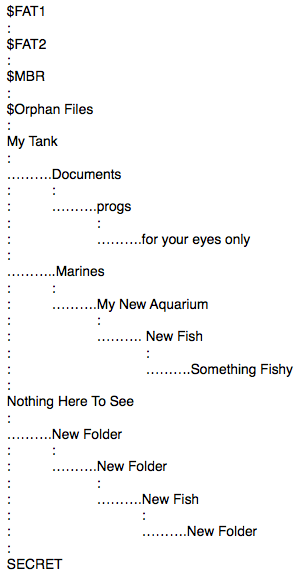
\includegraphics[width=5cm]{Images/DirectoryStructure.png}
					\caption{Directory Structure}
				\end{figure}

				\begin{figure}[ht!]
					\centering
					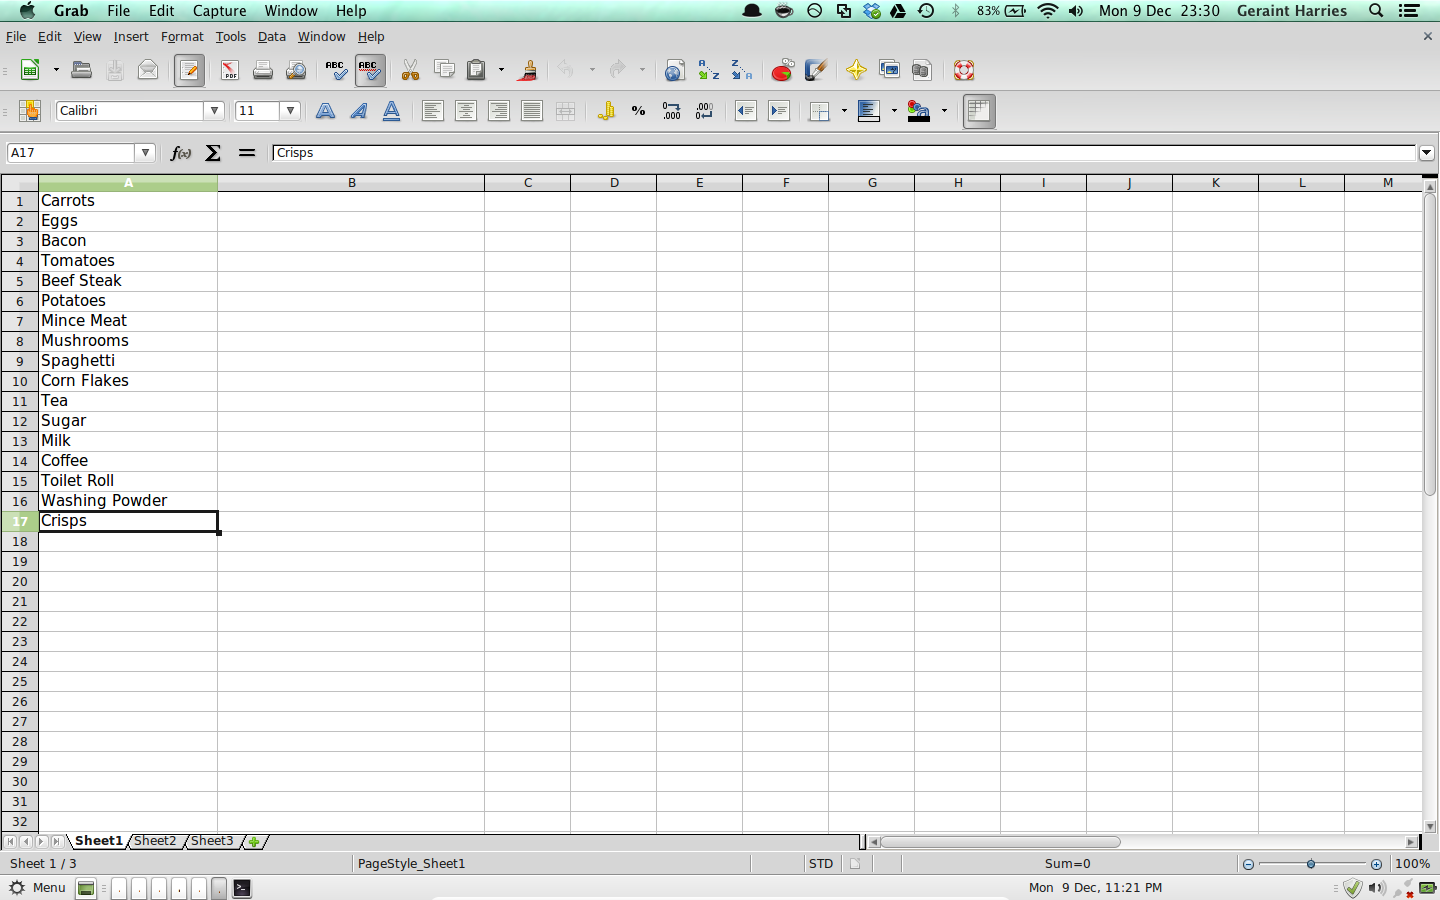
\includegraphics[width=12cm]{Images/ShoppingListExcel.png}	
					\caption{Shopping List.xls with .xls at the end}
				\end{figure}

				\begin{figure}[ht!]
					\centering
					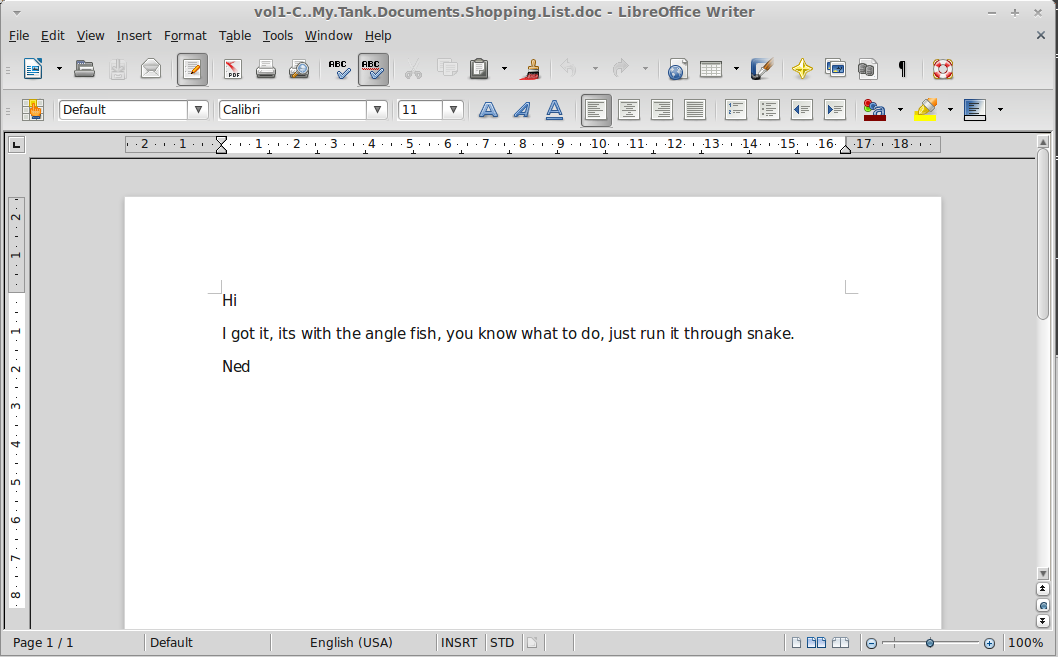
\includegraphics[width=12cm]{Images/ShoppingListWord.png}
					\caption{Shopping List.xls with .doc at the end i.e. Shopping List.doc}
				\end{figure}

				\begin{figure}[ht!]
					\centering
					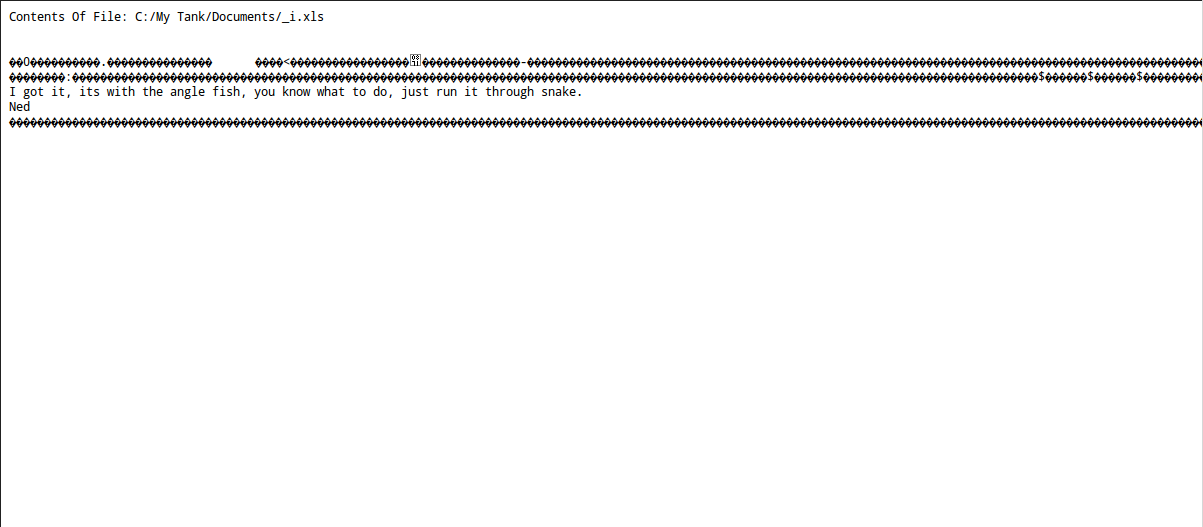
\includegraphics[width=12cm]{Images/_i.png}
					\caption{\_i.xls}
				\end{figure}

				\begin{figure}[ht!]
					\centering
					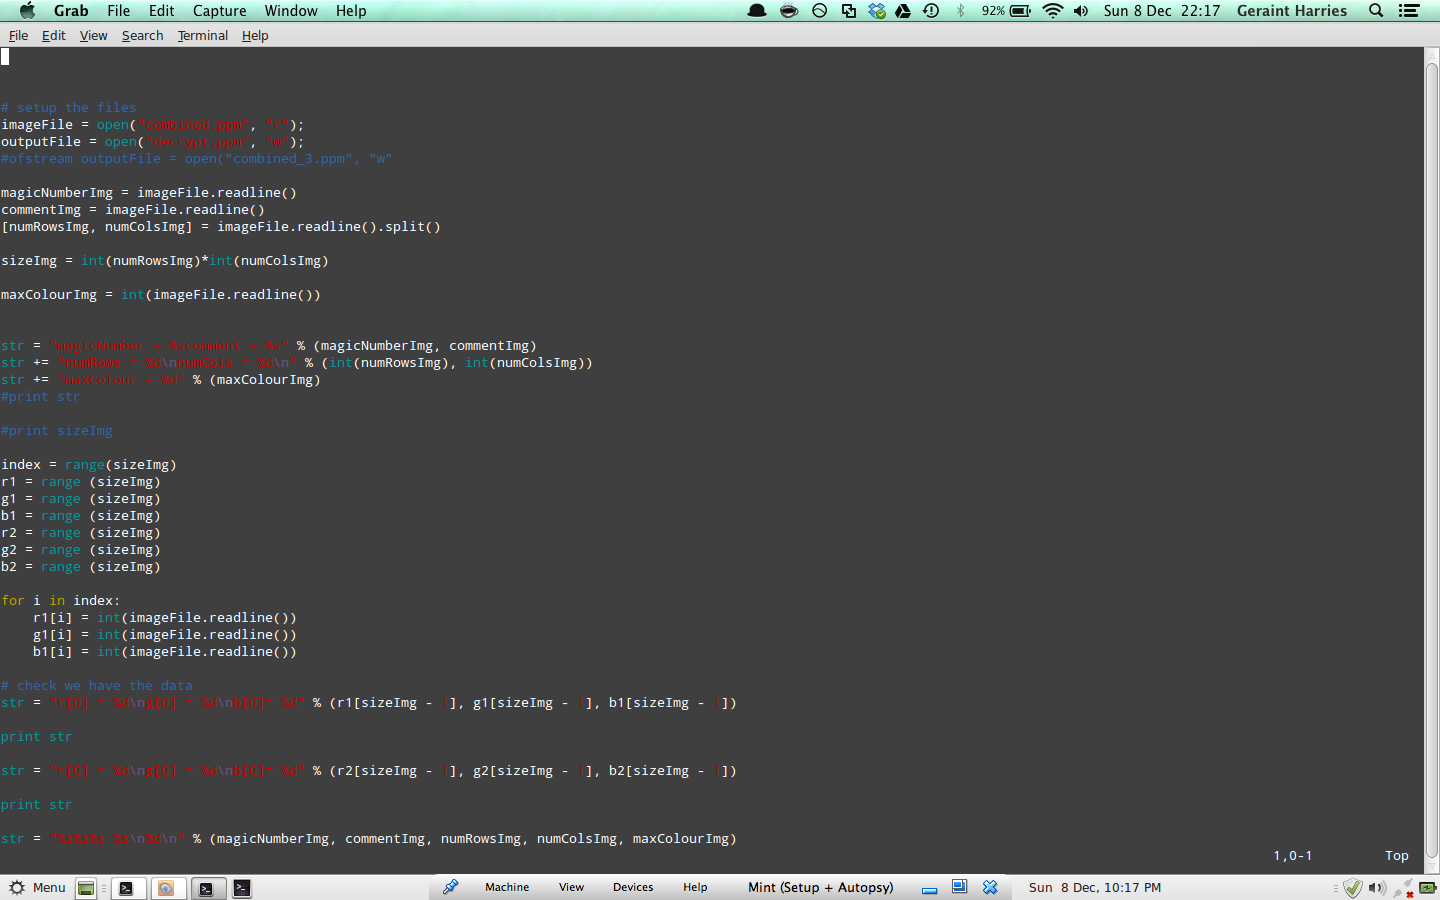
\includegraphics[width=12cm]{Images/_nape1.png}
					\caption{\_nake Page 1}
				\end{figure}

				\begin{figure}[ht!]
					\centering
					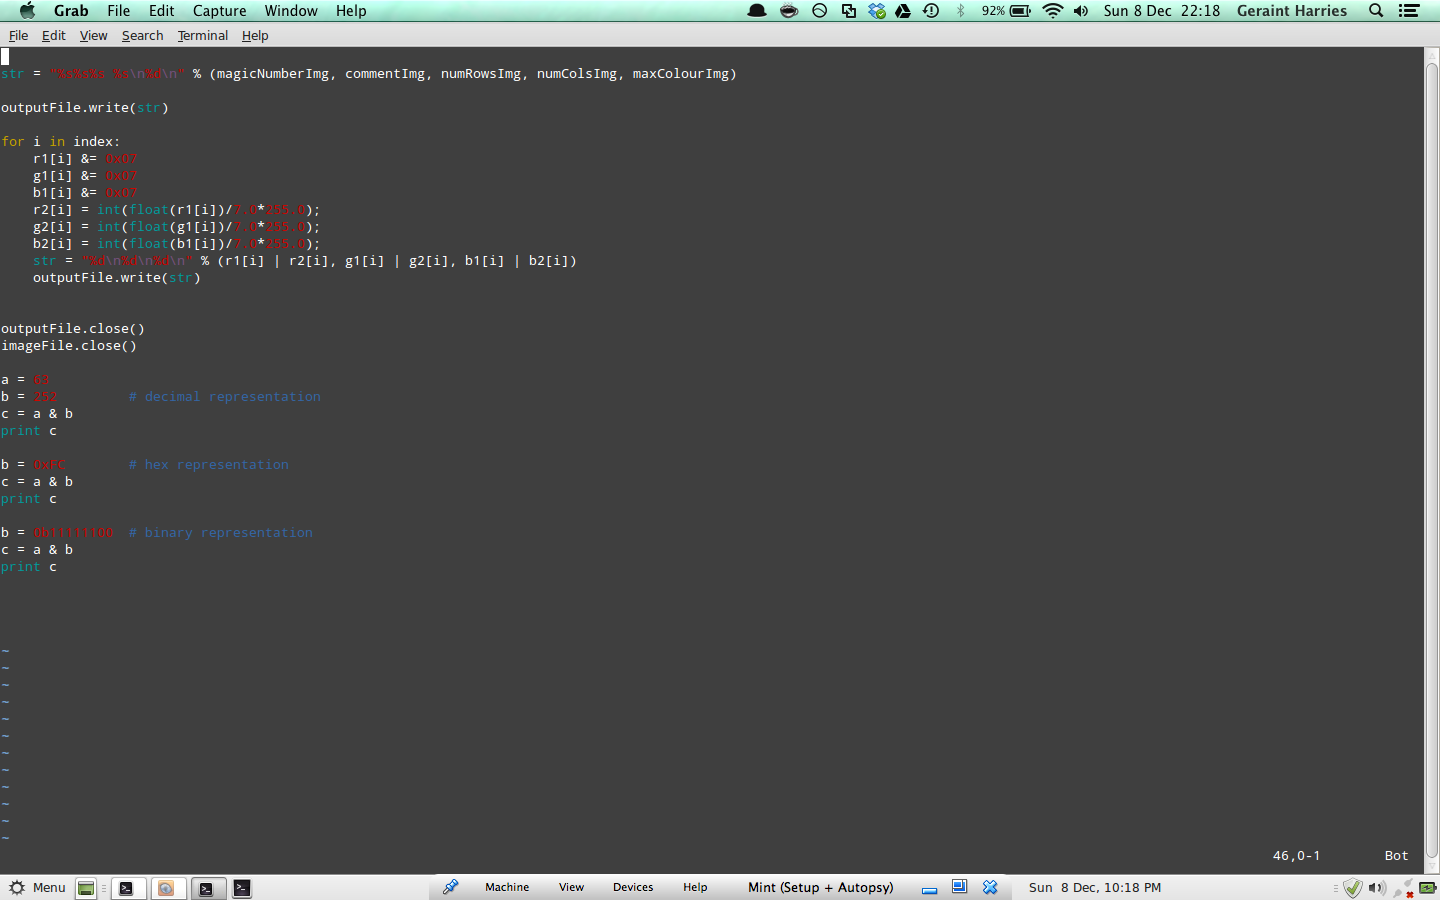
\includegraphics[width=12cm]{Images/_nape2.png}
					\caption{\_nake Page 2}
				\end{figure}
				
				\begin{figure}[ht!]
					\centering
					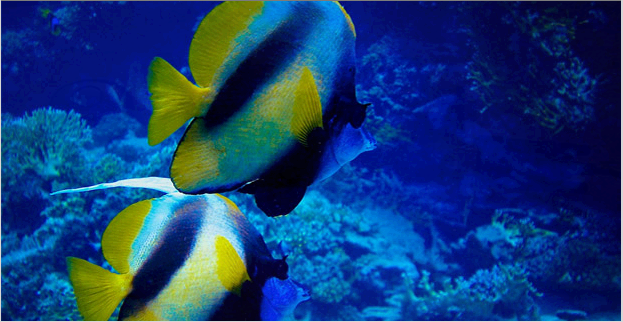
\includegraphics[width=12cm]{Images/_ombinedPng.png}
					\caption{\_ombined.png}
				\end{figure}
				\begin{figure}[ht!]
					\centering
					
\includegraphics[width=12cm]{Images/_ombinedPpm.png}
					\caption{\_ombined.ppm}
				\end{figure}
				\begin{figure}[ht!]
					\centering
					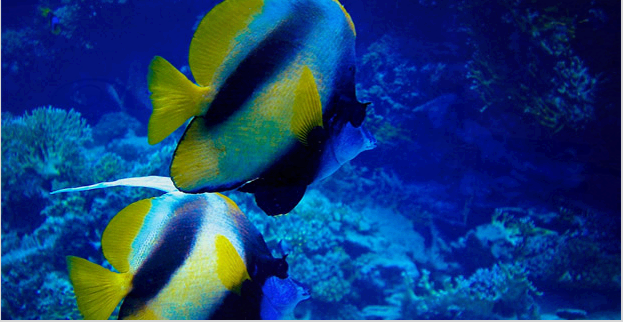
\includegraphics[width=12cm]{Images/AngleFishPpm.png}
					\caption{AngleFish.ppm}
				\end{figure}

				\begin{figure}[ht!]
					\centering
					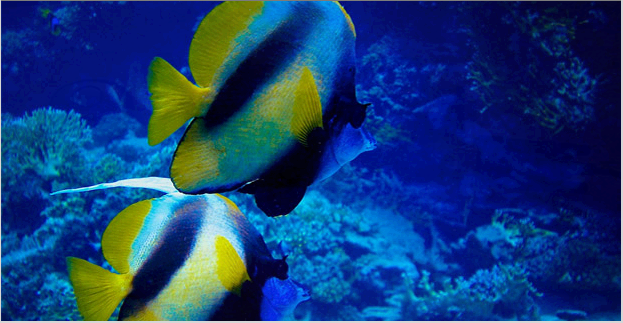
\includegraphics[width=12cm]{Images/AngleFishPng.png}
					\caption{AngleFish.png}
				\end{figure}

				\begin{figure}[ht!]
					\centering
					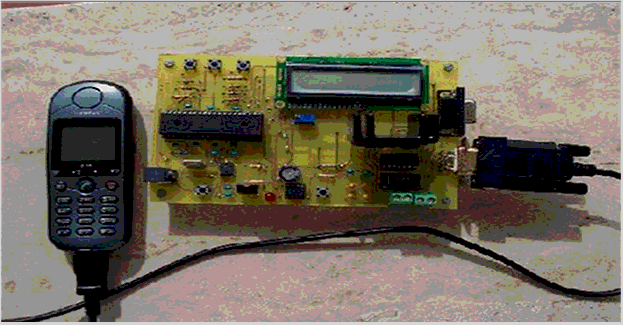
\includegraphics[width=12cm]{Images/decrypt.png}
					\caption{This image was generated by running AngleFish.ppm through the \_nake.py script}
				\end{figure}

	\end{document}
